\begin{frame}
\frametitle{Le travail effectu�}
\framesubtitle{Plate-forme de tests (1/5)}
	\begin{block}{Objectif}
        �valuer la performance de carte acoustique Version 4G
	\end{block}

	\begin{exampleblock}{Proc�dure}
	\textbf{Phase 1:} Plan du test\\
	\textbf{Phase 2:} D�marrage du test\\
	\textbf{Phase 3:} Analyse des r�sultats
	\end{exampleblock}

\end{frame}

% ------------------------- %
\begin{frame}
\frametitle{Le travail effectu�}
\framesubtitle{Plate-forme de tests (2/5)}

\begin{columns}
\begin{column}[l]{0.6\textwidth}
	\begin{exampleblock}{Plan du test}
\textbf{TEST 1:} Fiabilit� de l'encryptage\\
\textbf{TEST 2:} Fiabilit� �mission sonore\\
\textbf{TEST 3:} Consommation\\
\textbf{TEST 4:} Dur�e de vie\\
\textbf{TEST 5:} R�cup�ration via IPad\\
\textbf{TEST 6:} R�cup�ration via IPhone\\
\textbf{TEST 7:} R�cup�ration via Windows
	\end{exampleblock}
\end{column}
\begin{column}[r]{0.4\textwidth}
	\begin{exampleblock}{Facteurs}
\begin{itemize}
\item Distances
\item Importance
\item P�riph�riques
\item Environnements
\item Versions
\item Phases
\item Nombre de tests
\item Logiciel utilis�
\end{itemize}
	\end{exampleblock}
\end{column}
\end{columns}
\end{frame}

% ------------------------- %
\begin{frame}
\frametitle{Le travail effectu�}
\framesubtitle{Plate-forme de tests (3/5)}
	\begin{figure}
	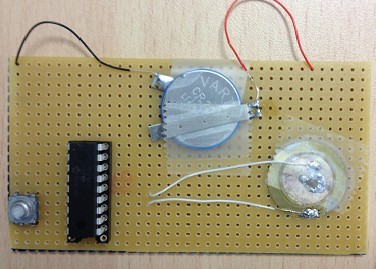
\includegraphics[width=0.5\textwidth]{images/p1}	
	%\caption{Prototype utilis�}
	\end{figure}
\begin{exampleblock}{Strat�gie}
\textbf{Le prototype:} g�n�re une s�quence de 100 messages acoustiques
\end{exampleblock}
\end{frame}

% ------------------------- %
\begin{frame}
\frametitle{Le travail effectu�}
\framesubtitle{Plate-forme de tests (4/5)}

\begin{exampleblock}{Strat�gie}
\textbf{Le prototype:} g�n�re une s�quence de 100 messages acoustiques
\end{exampleblock}

\begin{block}{Environnement du code source}
\begin{itemize}
\item IDE: MPLAB V.8
\item Language: Assembleur
\item Compilateur: MPASM
\item Microcontr�leur: PIC16F648A (Microchip)
\begin{itemize}
\item 256 octets RAM
\item 4096 mots flash
\item communication usart uniquement
\item 1 vecteur interruption
\end{itemize}
\end{itemize}
\end{block}
\end{frame}

% ------------------------- %
\begin{frame}
\frametitle{Le travail effectu�}
\framesubtitle{Plate-forme de tests (5/5)}

\begin{block}{Analyse des r�sultats}
\begin{itemize}
\item Traitement statistique des r�sultats
\item Analyse de l�effet filtrage sous PC
\item Analyse de volume de son par sonom�tre
\item Diff�rences entre les prototypes et les cartes
\item Analyse de l�effet environnement
\end{itemize}
\end{block}
\end{frame}








